First, we used the reference count's timestamps as bins. One bin covers a timespan of 5 minutes.
If there are multiple count of a group in one bin, we calculated the average.
Because there are about 1900 bins for these 4 days, an offset of 3 or 4, to the reference, results in a high absolute
difference of about 10000.
We can see in figure \ref{fig_comparison} and \ref{fig_comparison2} the group's count compared to the reference count.
To compare the group's counting algorithm performance better, we calculated the absolute
difference to the reference count. Null values were replaced by zero for this calculation.\\
Resulting, group 15 had the best performance and our counting algorithm (group 8) is on the
third place for the metric absolute distance.

\begin{figure}
    \centering
    \begin{subfigure}[b]{0.45\textwidth}
        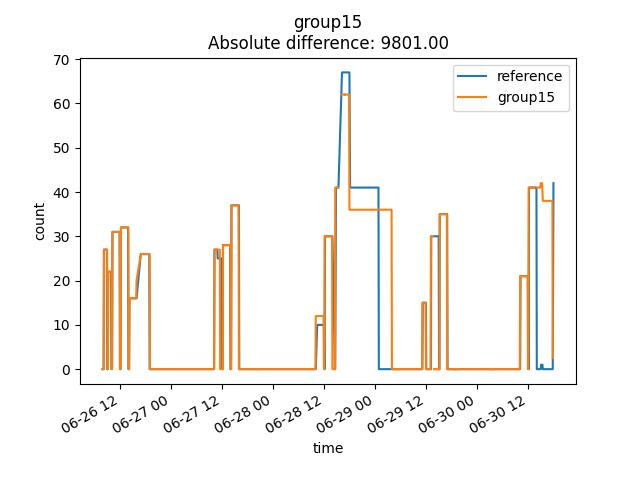
\includegraphics[width=\linewidth]{figures/ref-group15.jpeg}
        \caption{Place 1 of 9}
    \end{subfigure}
    \begin{subfigure}[b]{0.45\textwidth}
        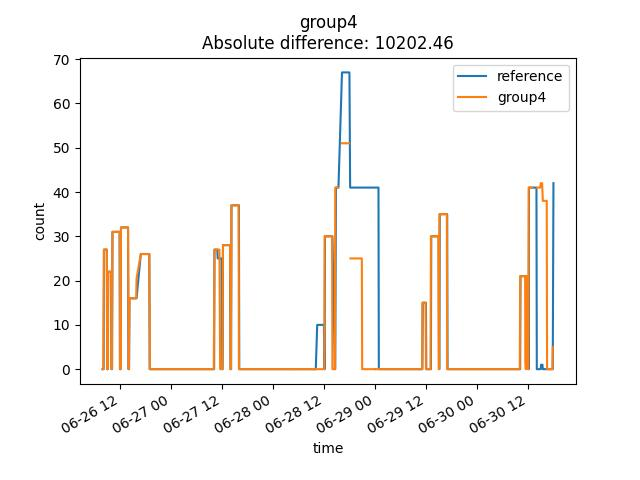
\includegraphics[width=\linewidth]{figures/ref-group4.jpeg}
        \caption{Place 2 of 9}
    \end{subfigure}

    \begin{subfigure}[b]{0.45\textwidth}
        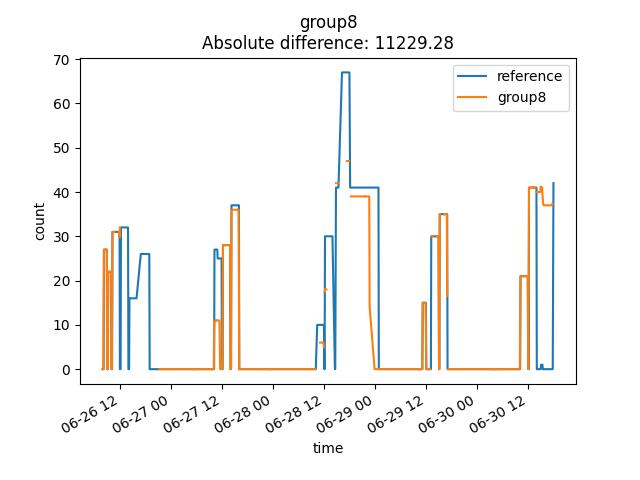
\includegraphics[width=\linewidth]{figures/ref-group8.jpeg}
        \caption{Place 3 of 9}
    \end{subfigure}
    \begin{subfigure}[b]{0.45\textwidth}
        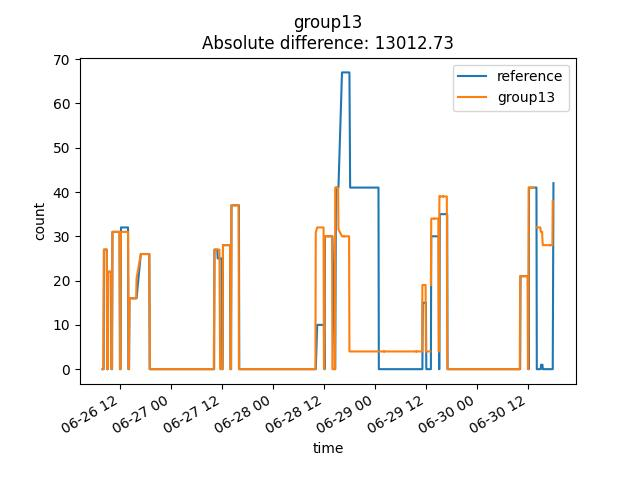
\includegraphics[width=\linewidth]{figures/ref-group13.jpeg}
        \caption{Place 4 of 9}
    \end{subfigure}

    \begin{subfigure}[b]{0.45\textwidth}
        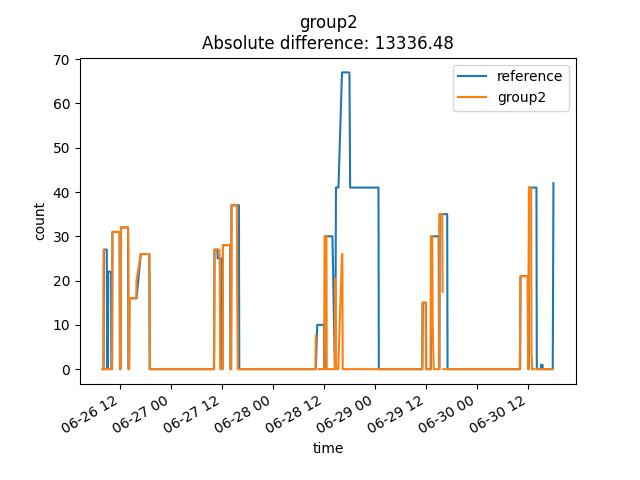
\includegraphics[width=\linewidth]{figures/ref-group2.jpeg}
        \caption{Place 5 of 9}
    \end{subfigure}
    \begin{subfigure}[b]{0.45\textwidth}
        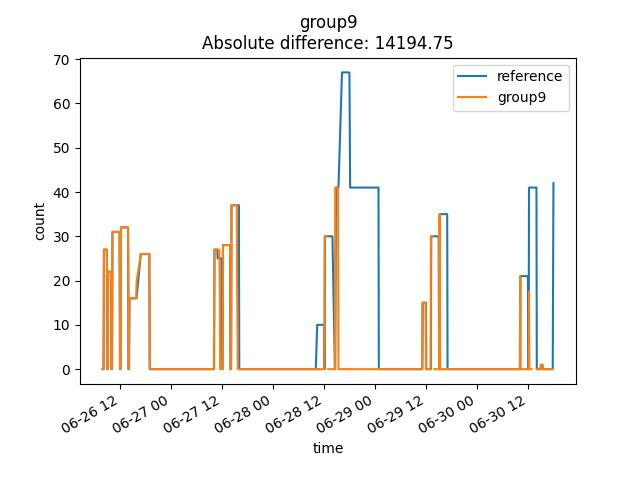
\includegraphics[width=\linewidth]{figures/ref-group9.jpeg}
        \caption{Place 6 of 9}
    \end{subfigure}

    \caption{Group comparison. The absolute difference (in seconds) is the absolute difference to the reference count.
        The pictures are ordered descending by their counting algorithm performance.}
    \label{fig_comparison}
\end{figure}

\begin{figure}
    \center
    \begin{subfigure}[b]{0.45\textwidth}
        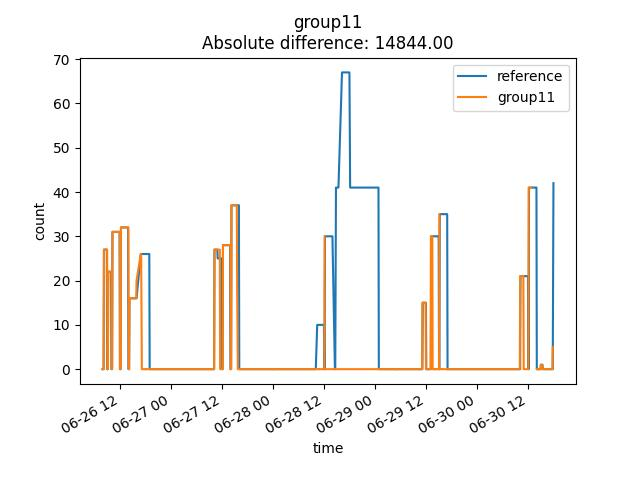
\includegraphics[width=\linewidth]{figures/ref-group11.jpeg}
        \caption{Place 7 of 9}
    \end{subfigure}
    \begin{subfigure}[b]{0.45\textwidth}
        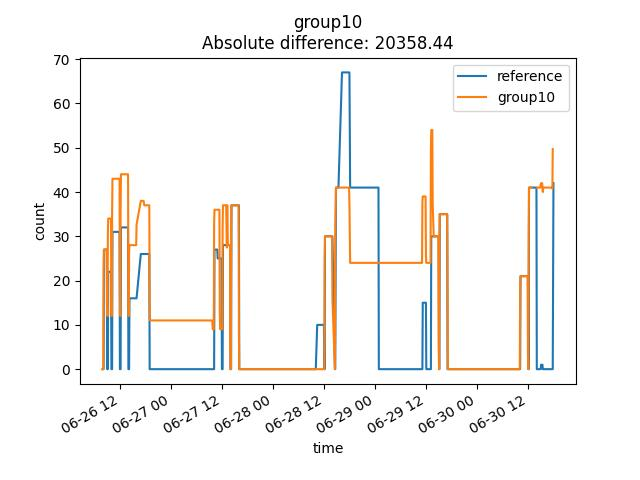
\includegraphics[width=\linewidth]{figures/ref-group10.jpeg}
        \caption{Place 8 of 9}
    \end{subfigure}

    \begin{subfigure}[b]{0.45\textwidth}
        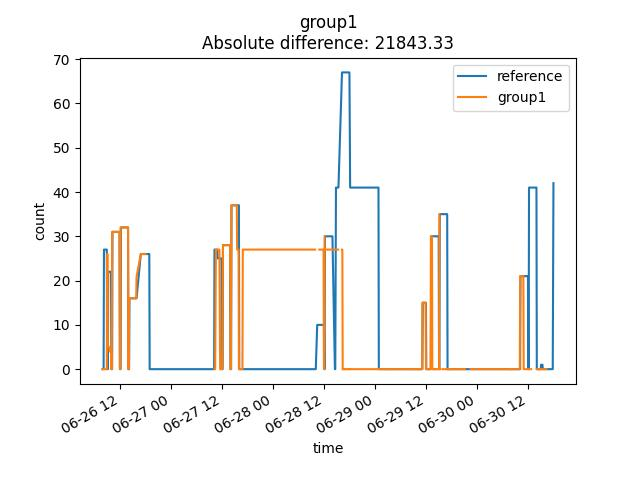
\includegraphics[width=\linewidth]{figures/ref-group1.jpeg}
        \caption{Place 9 of 9}
    \end{subfigure}
    \caption{Group comparison. The absolute difference (in seconds) is the absolute difference to the reference count.
        The pictures are ordered descending by their counting algorithm performance.}
    \label{fig_comparison2}
\end{figure}